\documentclass[11pt]{article}            % Report class in 11 points
\parindent0pt  \parskip10pt             % make block paragraphs
\usepackage{graphicx}
\usepackage{listings}
\graphicspath{ {images/} }
\usepackage{graphicx} %  graphics header file
\begin{document}
\begin{titlepage}
    \centering
  \vfill
    
\includegraphics[width=8cm]{uni_logo.png} \\ 
	\vskip2cm
    {\bfseries\Large
	Data Structures and algorythm  \\ (CS09203)\\
	
	\vskip2cm
	Lab Report 
	 
	\vskip2cm
	}    

\begin{center}
\begin{tabular}{ l l  } 

Name: & MuhammadTalhaKhalid \\ 
Registration \#: &CSU-S16-135\\ 
Lab Report \#: &5\\ 
 Dated:& 16-04-2018\\ 
Submitted To:& Mr. Usman Ahmed\\ 

 %\hline
\end{tabular}
\end{center}
    \vfill
    The University of Lahore, Islamabad Campus\\
Department of Computer Science \& Information Technology
\end{titlepage}

    {\bfseries\Large
\centering
	Experiment \# 3 \\
Inserti and deletion in Link list\\
	
	}    
 \vskip1cm
 \textbf {Objective}\\  How to insert and delete data from nodes in link list.
 
 \textbf {Software Tool} \\
1. Windows 8.1 \\
2. dev c++\\
3. c++\\

\section{Theory }              
In this experiment i insert 6 calues in link list and then delete the value from it.First of all it will check the root of the node if data entered is there it will delete it otherwise it will move to next node until given value is there or next node will be NULL \\
link list  has 3  rules:\\
1.	it has unlimited space.\\
2.	you can insert and delete nde easily.\\
3.       for deletion it will check 1st node then other till the nod is !=NULL \\


\section{Task}  
\subsection{Procedure: Task 1 }     

\begin{figure*}
\centering
  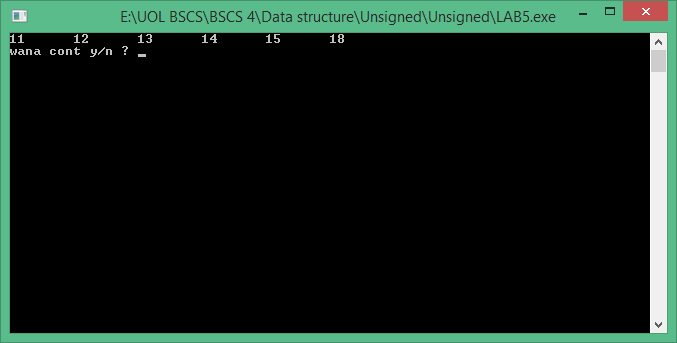
\includegraphics[width=12cm,height=6cm,keepaspectratio]{1.png}
\caption{6 elements in link list}
\label{Figure:1}    
  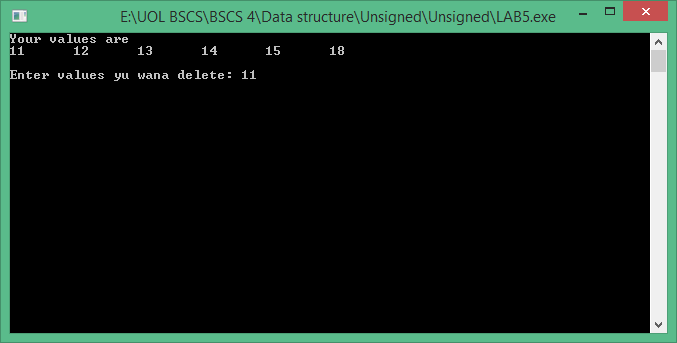
\includegraphics[width=12cm,height=6cm,keepaspectratio]{2.png}
\caption{delete 11 from link list}
\label{Figure:2}   
\end{figure*}
We can remove any number from that link list

\subsection{Procedure: Task 2 }     
\begin{lstlisting}[language=C++]
#include<stdio.h>
#include<iostream>
#include<dos.h>
#include<unistd.h>
#include<string>
#include<stdlib.h>
#include<menu.h>
#include <list>
using namespace std;
class Node {
public:
int val;
Node *next;	
Node() {
next=NULL;
val=0;	
}
};
class ll {
public:
Node *start,*temp, *newnode;	
ll() {
start=NULL;	
}
void addnode(int a) {
if(start==NULL) {
	temp=new Node;
	start=temp;
	temp->val=a;
}else {
	temp=start;
while(temp->next!=NULL) {
	temp=temp->next;
}	
newnode=new Node;
newnode->val=a;
temp->next=newnode;
}
}
void del(int n) {
	Node *prev;
	temp=start;
	if (start==NULL) {
	
		cout << "Nothing to delete, the list is empty!\n";
	} else if(temp->val==n) {
			start=temp->next; 
			delete temp;
			cout <<"value deleted\n";
			return ;
		} else {
		
		while (temp!=NULL) {
			if(temp->val==n) {
				cout <<"value deleted\n";
				prev->next=temp->next;
				delete temp;
				break;
			} else {
			
			prev=temp;
			temp=temp->next;
			}
		}
	}
	//	cout << "value not found!"<<endl;	
}
void ShowTime() {
Node *imp;
imp=start;	
while(imp!=NULL) {
cout<<imp->val<<"\t";
imp=imp->next;
}
cout<<endl;
}
};
int choice;
string subchoice="n";
int num;
void menu() {
system("cls");
cout<<"press 1 to enter data\n";
cout<<"press 2 to display data\n";
cout<<"press 3 to remove data\n";	
cout<<"press 4 to exit\n\n";
}
int main()
{
ll lo;
do {
menu();
cout<<"choose from above: ";
cin>>choice;
switch (choice) {
case 1:
do {
system("cls");
cout<<"Enter values: ";
cin>>num;	
lo.addnode(num);
cout<<"wana cont y/n ? ";
cin>>subchoice;	
}while(subchoice!="y");
break;
case 2:
system("cls");	
do {
lo.ShowTime();
cout<<"wana cont y/n ? ";
cin>>subchoice;	
}while(subchoice!="y");
break;
case 3:
system("cls");
do {
cout<<"Your values are\n";
lo.ShowTime();
cout<<"\nEnter values yu wana delete: ";
cin>>num;	
lo.del(num);
cout<<"wana exit y/n ? ";
cin>>subchoice;	
}while(subchoice!="y");
break;	
}
}while(choice!=4);
return 0;
}
\end{lstlisting}
\newpage
\begin{figure*}
\section{Output:}
\centering
  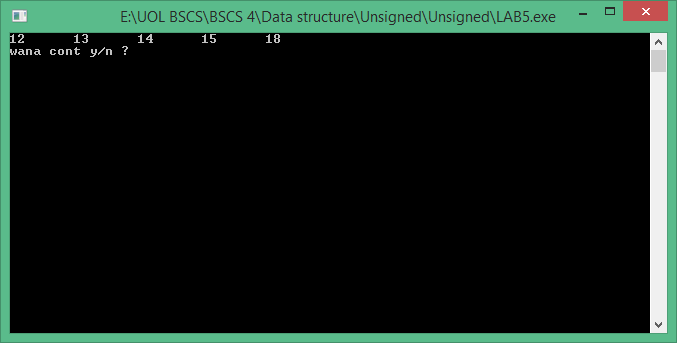
\includegraphics[width=12cm,height=6cm,keepaspectratio]{3.png}
\caption{Output of the program after deletion}
\label{Figure:3}     
\end{figure*}
\section{Conclusion}  
this is basic concept of how we add and remove nodes from link list using the address of the nodes linklist is basic concept about how to manage our data
\end{document}                          % The required last line
